% =====================================================================
% 3. Desenvolvimento
% Uma subseção por etapa do enunciado (itens 1 a 6). Cada uma fica em um arquivo
% em secoes/03-desenvolvimento/ e as imagens em figuras/03-desenvolvimento/<etapa>/.
% =====================================================================
\section{Desenvolvimento}\label{sec:desenvolvimento}

Esta seção explica cada passo do trabalho, na mesma ordem do enunciado: criar os objetos, montar
a cena, colocar a câmera, projetar em perspectiva, calcular a luz e pintar a imagem. O código foi
separado em arquivos, e cada arquivo cuida de uma parte, como mostra a
Tabela~\ref{tab:arquivos}.

\begin{table}[H]
  \centering
  \caption{Arquivos do código e suas funções}\label{tab:arquivos}
  \begin{tabularx}{\textwidth}{lX}
    \toprule
    Arquivo & O que faz \\
    \midrule
    \texttt{primitives.py} & formas simples (cilindro, esfera, caixa, etc.) e como juntá-las \\
    \texttt{modeling.py} & cria a malha de triângulos e define os cinco objetos \\
    \texttt{math\_3d.py} & matrizes de translação, escala, rotação, câmera e projeção \\
    \texttt{illumination.py} & cálculo da luz pelo modelo de Phong \\
    \texttt{rasterizer.py} & desenho de retas, preenchimento dos triângulos e cores \\
    \texttt{main.py} & monta a cena, roda todos os passos e mostra as imagens \\
    \bottomrule
  \end{tabularx}
  \fonte{Os autores (2026).}
\end{table}

% Etapa 1 do enunciado: modelagem dos 5 objetos.
% Fonte no código: primitives.py, modeling.py
% Função que retorna o sólido: modeling.criar_solido. Figuras: visualizar_objetos.py (salvas pelo botão de salvar da janela).
\subsection{Modelagem dos objetos}\label{sec:modelagem}

Os cinco objetos foram modelados cada um no seu sistema de coordenadas, apoiados em $y = 0$ e
centrados no eixo $y$. Só o haltere fica deitado, ao longo do eixo $x$.

Cada objeto é uma função $F(x, y, z)$ que vale menos que zero dentro do objeto, zero na superfície e
mais que zero fora. Formas simples (cilindro, cone, esfera, caixa e toro) são combinadas: a união é
o mínimo entre as funções e a subtração é $\max(A, -B)$, usada para deixar a lixeira oca. O
algoritmo \textit{Marching Cubes} \cite{lorensen1987}, da biblioteca scikit-image
\cite{vanderwalt2014}, recebe $F$ em uma grade de 80 pontos por eixo e devolve os triângulos de
$F = 0$.

A função \texttt{criar\_solido} devolve vértices, faces, arestas, normais das faces, normais dos
vértices e cor, tudo em coordenadas do objeto. As normais apontam para fora. Em todos os objetos, a
malha satisfaz $V - A + F = 2$, o que indica superfície fechada e sem buracos. A
Figura~\ref{fig:objetos} mostra os objetos com os eixos e as normais de algumas faces (setas
pretas), em uma grade de 50 pontos por eixo, mais leve para exibir. A cena usa 80 pontos.

\begin{figure}[H]
  \centering
  \caption{Objetos no sistema de coordenadas do objeto}\label{fig:objetos}
  \begin{subfigure}{0.31\textwidth}
    \centering
    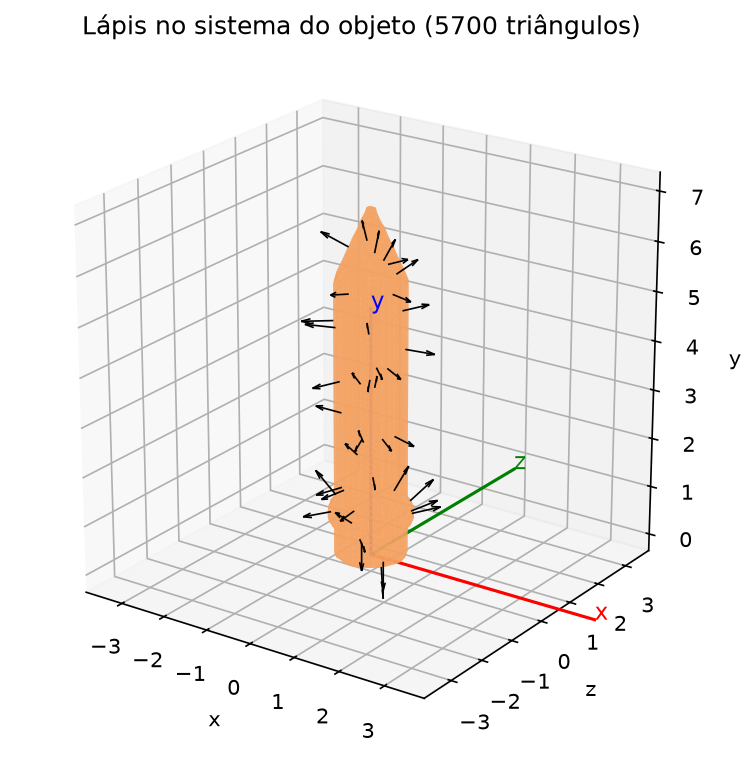
\includegraphics[width=\textwidth]{03-desenvolvimento/01-modelagem/lapis.png}
    \caption{Lápis}
  \end{subfigure}\hfill
  \begin{subfigure}{0.31\textwidth}
    \centering
    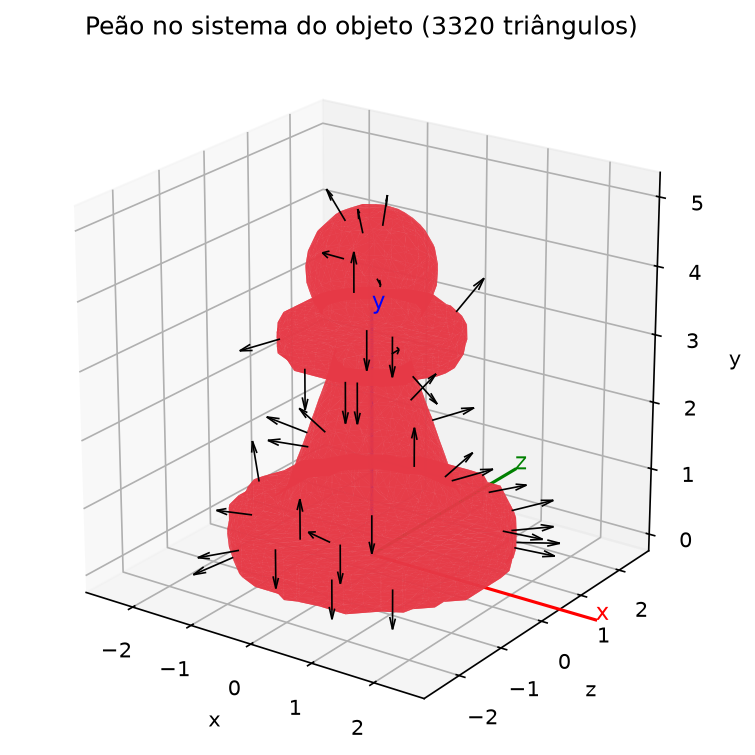
\includegraphics[width=\textwidth]{03-desenvolvimento/01-modelagem/peao.png}
    \caption{Peão}
  \end{subfigure}\hfill
  \begin{subfigure}{0.31\textwidth}
    \centering
    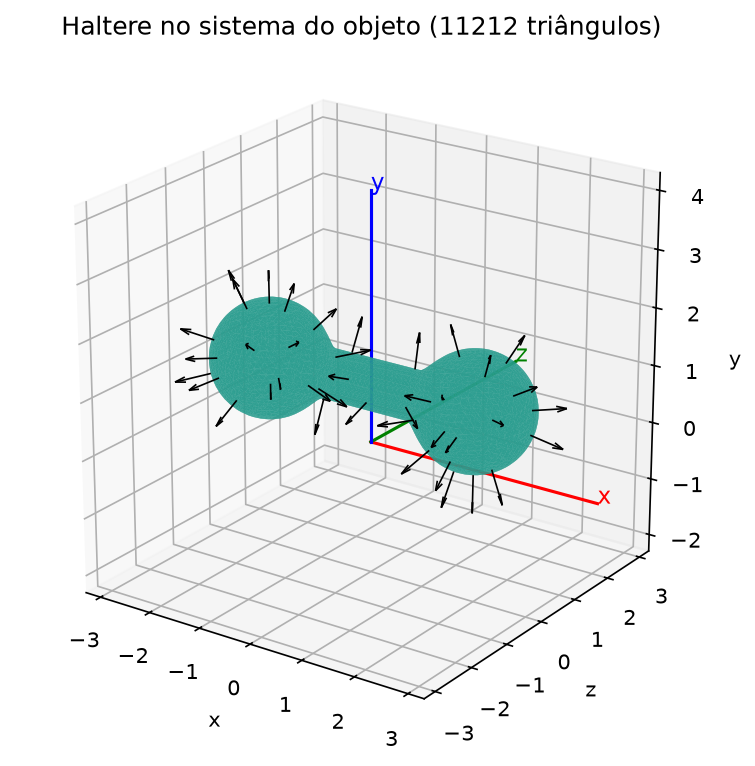
\includegraphics[width=\textwidth]{03-desenvolvimento/01-modelagem/haltere.png}
    \caption{Haltere}
  \end{subfigure}

  \vspace{6pt}
  \begin{subfigure}{0.31\textwidth}
    \centering
    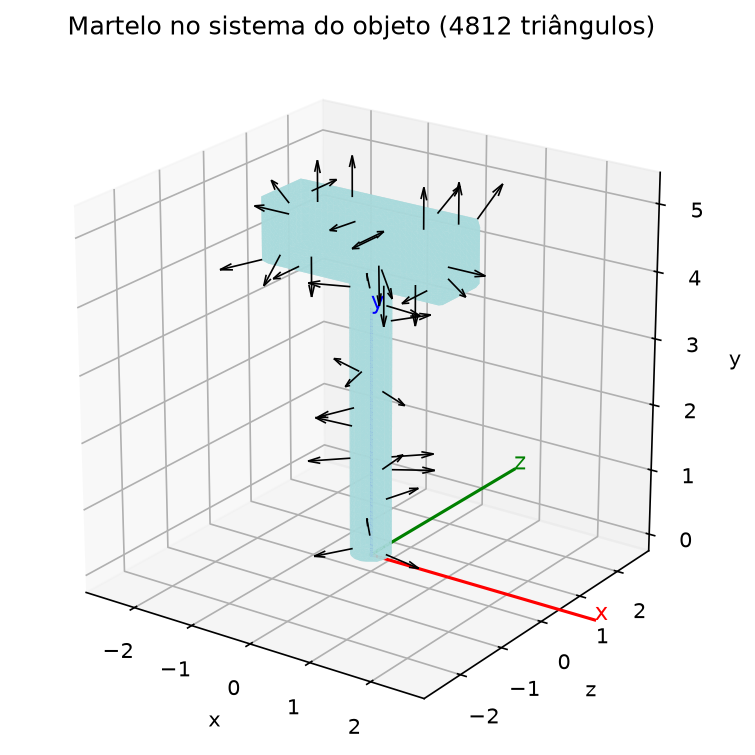
\includegraphics[width=\textwidth]{03-desenvolvimento/01-modelagem/martelo.png}
    \caption{Martelo}
  \end{subfigure}\hspace{0.04\textwidth}
  \begin{subfigure}{0.31\textwidth}
    \centering
    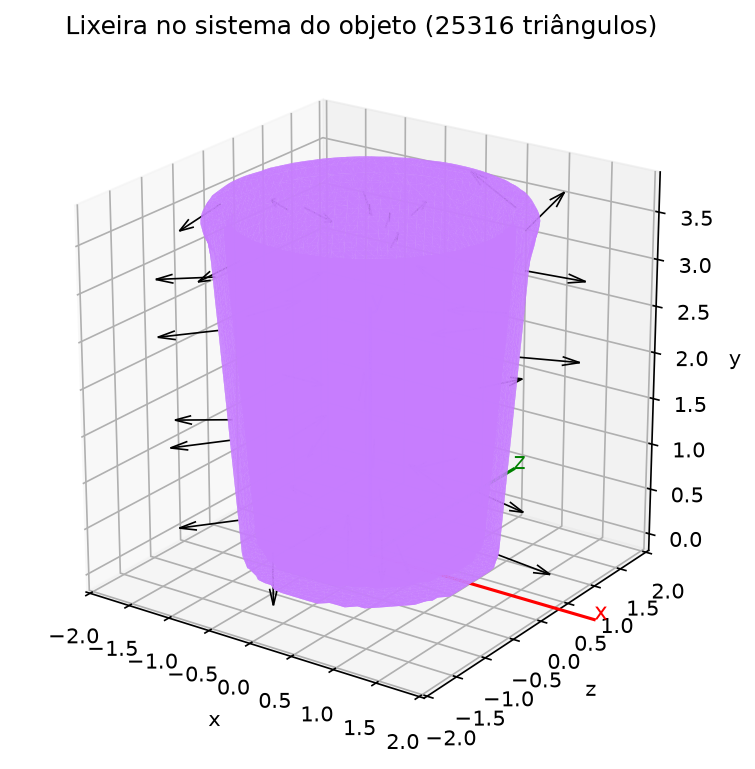
\includegraphics[width=\textwidth]{03-desenvolvimento/01-modelagem/lixeira.png}
    \caption{Lixeira}
  \end{subfigure}
  \fonte{Autoria própria (2026)}
\end{figure}

% Etapa 2 do enunciado: cena no sistema de coordenadas do mundo.
% Fonte no código: math_3d.py (translação, escala, rotações), main.py (CENA)
% Dica: matriz do mundo M = T R S, valores da cena, limite |10|, ausência de interseção.
% Figuras: cena 3D no mundo, em figuras/03-desenvolvimento/02-cena/.
\subsection{Composição da cena}\label{sec:cena}

\confirmar{escrever: transformações aplicadas a cada objeto (escala, rotação, translação) e tabela de posições}

\confirmar{escrever: como foi garantido o limite |10| e a ausência de sobreposição}

% Etapa 3 do enunciado: sistema de coordenadas da câmera.
% Fonte no código: math_3d.py (look_at), main.py (EYE_PRINCIPAL, EYE_BLENDER)
% Dica: eye, at, up, base (u, v, n), matriz de visualização, ponto da origem do mundo,
% mais de um valor de eye gerando novas imagens.
% Figuras: cena no sistema da câmera, em figuras/03-desenvolvimento/03-camera/.
\subsection{Sistema de coordenadas da câmera}\label{sec:camera}

\confirmar{escrever: cálculo da base vetorial a partir de eye, at e up}

\confirmar{escrever: transformação mundo para câmera e marcação da origem do mundo}
\confirmar{escrever: exemplos com valores diferentes de eye}

% Etapa 4 do enunciado: projeção em perspectiva.
% Fonte no código: math_3d.py (projecao_perspectiva, divisao_perspectiva), main.py (ndc_para_pixel)
% Figura do item 4a: visualizar_projecao.py (salva pelo botão de salvar da janela).
\subsection{Projeção em perspectiva}\label{sec:projecao}

Na projeção em perspectiva, objetos mais distantes aparecem menores \cite{azevedo2018}. O volume de
visão é definido pelo ângulo de abertura vertical ($fov = 58^\circ$), pela proporção da janela
($1$) e pelas distâncias dos planos próximo ($0{,}1$) e distante ($100$). Dele sai o valor
$f = \cot(fov/2)$, que corresponde ao $d$ da aula: a posição projetada é

\begin{equation}
  x' = d \cdot \frac{x}{z} .
\end{equation}

Como $z$ está no denominador, quanto mais longe o ponto, mais perto do centro ele fica. No código,
essa conta é feita com uma matriz $4 \times 4$ e uma divisão final pela coordenada $w$. O resultado
são coordenadas entre $-1$ e $1$, que depois são convertidas em pixels da janela de projeção.
Triângulos fora do volume de visão ou voltados para trás não são iluminados nem rasterizados
(Seção~\ref{sec:rasterizacao}). A Figura~\ref{fig:projecao} mostra, à esquerda, os sólidos em 3D
no sistema da câmera com a janela de projeção e, à direita, a janela vista de frente.

\figura{03-desenvolvimento/04-projecao/eye1.png}{\textwidth}{Sólidos em 3D e projeção na janela, com $eye = (9{,}75;\ 13;\ 6{,}5)$}{fig:projecao}{Autoria própria (2026)}

% Etapa 5 do enunciado: iluminação.
% Fonte no código: illumination.py
% Dica: modelo de Phong \cite{phong1975}, componentes ambiente, difusa e especular,
% coeficientes (ka, kd, ks, brilho), posição da luz, cálculo por vértice.
% Figuras: opcional, comparação das componentes, em figuras/03-desenvolvimento/05-iluminacao/.
\subsection{Iluminação}\label{sec:iluminacao}

\confirmar{escrever: equação do modelo de Phong e valores usados}

\confirmar{escrever: como o RGB de cada vértice é calculado}

% Etapa 6 do enunciado: rasterização.
% Fonte no código: rasterizer.py, main.py
% Dica: eliminação de faces ocultas (normal da face e eixo z da câmera), retas (livro-texto,
% subseção 5.2.1), polígonos (par-ímpar com scan line), coordenadas baricêntricas, Z-buffer,
% 3 resoluções.
% Figuras: algoritmo em pseudocódigo ou diagrama, em figuras/03-desenvolvimento/06-rasterizacao/.
\subsection{Rasterização}\label{sec:rasterizacao}

\confirmar{escrever: eliminação de faces ocultas pela normal e pelo eixo z da câmera}

\confirmar{escrever: rasterização de retas e do preenchimento par-ímpar com scan line}

\confirmar{escrever: interpolação baricêntrica da cor e uso do Z-buffer}

